\chapter{Linux auf x86 vs. z Systems}
\label{cha:Unterschiede}

In den folgenden Abschnitten werden einige wichtige Unterschiede zwischen einem Linux fuer x86 und Linux on z behandelt.

\section{Workload Management}

Die IBM z Systems haben ein nahezu perfektes Workload Management.
Mit Linux on z wird auf einem Mainframe von ziemlich simplen Konzepten gebrauch gemacht, um den Workload zu optimieren
und zwischen High- und Low- Priority Workload zu unterscheiden:

\begin{description}
    \item[Identifizieren des Workloads]{Es muss identifiziert werden, was die Workloads sind die laufen.}
    \item[Messen wie lange diese Workloads dauern]{Es muss gemessen werden, wie lange diese Workloads dauern.}
    \item[Ausfindig machen der Uebergabe Punkten]{Wenn man herausgefunden hat, was die Workloads sind und wie lange diese dauern, kann begonnen werden diese zu optimieren.}
\end{description}

\newpage
Diese Workload Management Konzepte fuehren dazu, dass mit Linux on z die volle Prozessleistung genutzt werden kann (high utilitzation).

\begin{figure}[h!]
\centering
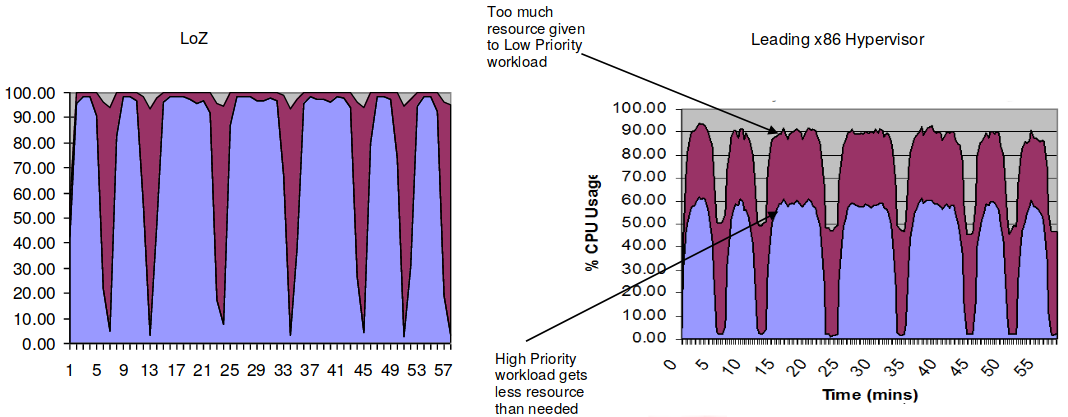
\includegraphics[width=.95\textwidth]{difference-workload-management}
\caption{Workload Management Vergleich mit x86\cite{WorkloadManagement}.}
\label{fig:WorkloadManagement}
\end{figure}

\section{Konsolidierung von Linux Servern}

In Rechenzentren hat man oft das Ziel, die Unterhaltungskosten und Effizienz zu optimieren.
Nicht nur was Platz und Strom angeht sondern auch die Effizienz und Auslastung der Server.
Ein IBM Mainframe mit Linux on z ist predestiniert dafuer komplette Linux Server Farmen auf einer
einzelnen Hardware zu konsolidieren.
Damit es sich ueberhaupt lohnt eine solche Konsolidierung in Betracht zu ziehe, braucht man eine kritische Masse
an Linux Servern. IBM illustriert diese \textit{kritische Masse} wie folgt:

\begin{figure}[h!]
\centering
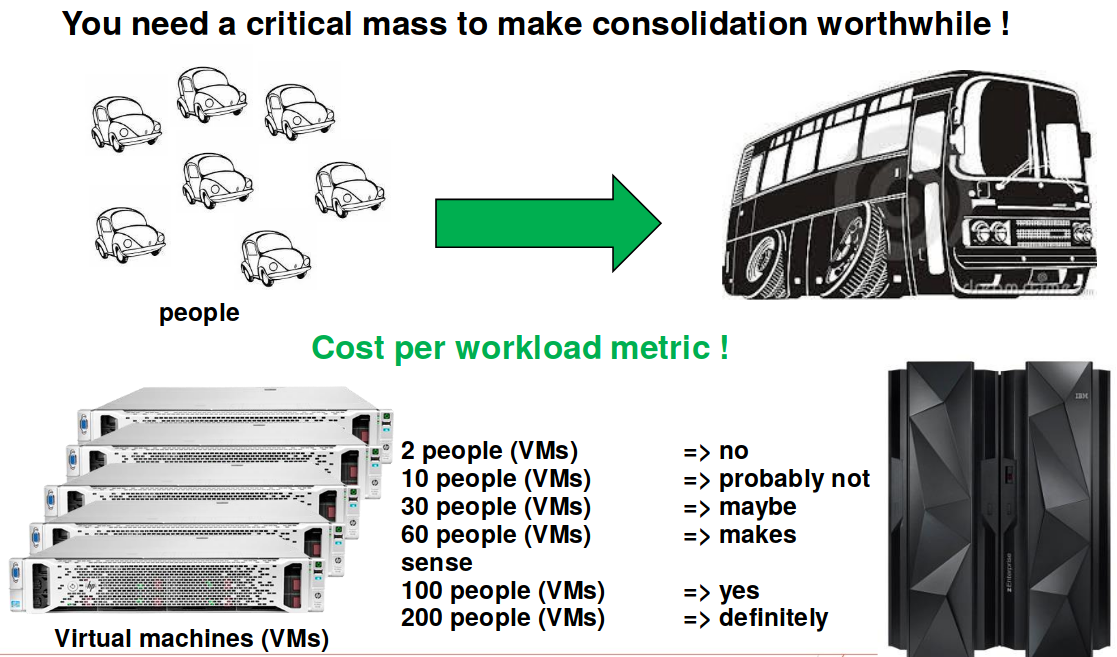
\includegraphics[width=.80\textwidth]{difference-kritische-masse}
\caption{Kritische Masse fuer Konsolidierung\cite{KonsolidierungKritischeMasse}.}
\label{fig:KonsolidierungKritischeMasse}
\end{figure}

IBM hat laut mehreren \textit{Eagle studies} folgende Statistik aufgestellt im Bezug auf x86-Cores zu Linux on z-Cores:

\begin{figure}[h!]
\centering
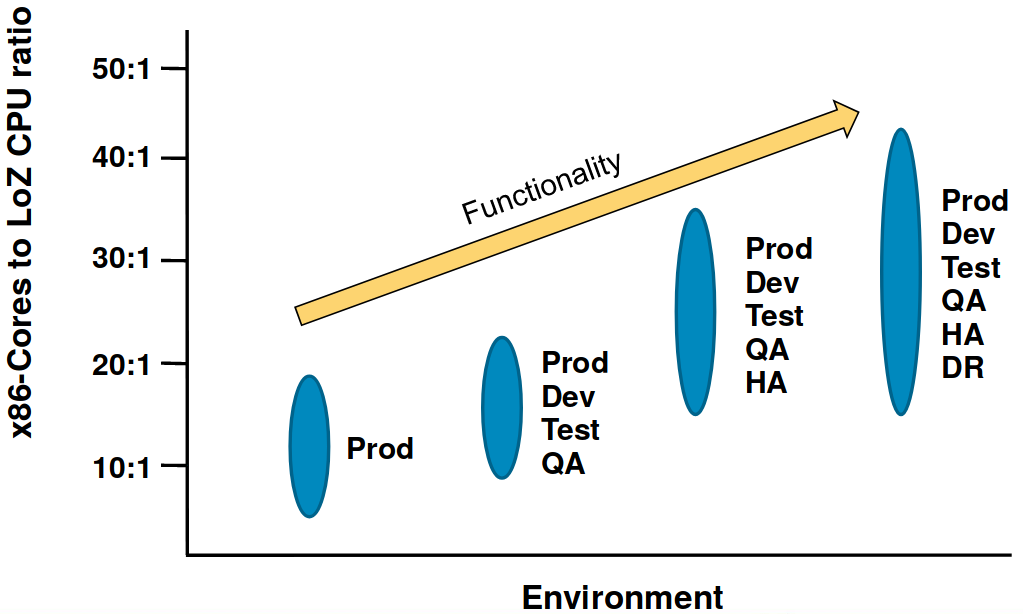
\includegraphics[width=.80\textwidth]{difference-cpu-ratio}
\caption{Rate von x86-Cores zu LoZ-Cores\cite{CPURatio}.}
\label{fig:CPURatio}
\end{figure}

Diese Statistik zeigt, dass umso komplexer ein Environment wird, umso mehr x86-Cores werden im Vergleich zu Linux on z-Cores gebraucht,
damit das Environment die erforderlichen Leistungen erbringen kann.

Dies ist vorallem auf die gute Leistung des Workload Managements zurueckzufuehren.

\section{Kommunikation ueber HiperSockets}
